% --------------------------------------------------------------------------
% Template for DCASE 2017 paper; to be used with:
%          dcase2017.sty  - DCASE 2017 LaTeX style file, and
%          IEEEbib.bst - IEEE bibliography style file.
% Adapted from spconf.sty and waspaa15.sty
% --------------------------------------------------------------------------

\documentclass{article}
\usepackage{dcase2017,amsmath,graphicx,url,times,booktabs, tabularx}
%\usepackage{color}
\usepackage{multicol}        % used for the two-column index
% Example definitions.
% --------------------
\def\defeqn{\stackrel{\triangle}{=}}
\newcommand{\symvec}[1]{{\mbox{\boldmath $#1$}}}
\newcommand{\symmat}[1]{{\mbox{\boldmath $#1$}}}

% Title.
% --------------------
\title{A HIERARCHIC MULTI-SCALED APPROACH FOR RARE SOUND EVENT DETECTION}

% Authors in two lines, use in case of many authors with many affiliations (uncomment and modify).
% --------------------
 \name{Fabio Vesperin,
       Diego Droghini,
       Daniele Ferretti,
       }
 \secondlinename{	
 	   Emanuele Principi,  
       Leonardo Gabrielli,
       Stefano Squartini, 
       Francesco Piazza
       }
       % fixed *.sty to allow names on multiple lines
 \address{Department of Information Engineering, Universit\`{a} Politecnica delle Marche, Ancona, Italy,\\ \{d.droghini, f.vesperini, d.ferretti\}@pm.univpm.it\\   
 		\{e.principi, l.gabrielli, s.squartini, f.piazza\}@univpm.it\\       
}
  

\begin{document}

\ninept
\maketitle

\begin{sloppy}

\begin{abstract}
We propose a system for rare sound event detection using hierarchical and multi-scaled approach based on Multi Layer Perceptron (MLP) and Convolutional Neural Networks (CNN). 
It is our contribution to the rare sound event detection task of the IEEE AASP Challenge on  Detection and Classification of Acoustic Scenes and Events (DCASE2017). The task consists on detection of event onset from artificially generated mixtures. Acoustic features are extracted from the acoustic signals, successively first event detection stage is performed by an MLP based neural network which proposes contiguous blocks of frames to the second stage. The CNN refines the event detection of the prior network, intrinsically operating on a multi-scaled resolution and discarding blocks that contain background wrongly classified by the MLP as event. Finally the effective onset time of the active event is obtained.
The achieved overall error rate and F-measure are respectively equal to 0.18 and 90.9\% on the development dataset and equal to 0.33 and 83.9\% on the evaluation dataset.	
\end{abstract}

\begin{keywords}
DCASE2017, Rare sound event detection, MLP, CNN, \textit{LogMel}
\end{keywords}


\section{Introduction}
\label{sec:intro}
%2 aprole su soude evet det
%2 parole su nostri lavori novelty + (fall detection)
%2 parole su dcase daaset + ref a loro


The field of computational auditory scene analysis (CASA) covers many topics. 
Nowadays, one of the most important topic is the automatic sound event detection (SED). 
SED is defined as the task of analysing a continuous audio signal in order to extract a description of the sound events occurring in the audio stream. This description is commonly expressed as a label that marks the start, the ending, and the nature of the occurred sound (e.g., children crying, cutlery, glass jingling).
Task 2 of DCASE challenge 2017 \cite{dcase2017web} consists in determining the precise onset time of three types of sounds: ``babycry'', ``glassbreak'' and ``gun shot'' eventually present in artificially generated audio sequences. The background audio material belongs to the TUT Acoustic Scenes 2016 dataset and it contains recordings from 15 different audio scenes.

\section{Proposed Method}
\label{sec:proposed-meth}
%algo composto da 4 stadi principali: eat extr - event detection - multiscaled detection refinement - event onset annotation 
The proposed system is a hierarchical algorithm composed of four main stages: the acoustic features extraction, the first event detection stage performed by a Multi Layer Perceptron Neural Network (MLP) and a dedicated smoothing procedure of its output. Then, a refinement of the previous decision stage is performed by a Convolutional Neural Network (CNN) which intrinsically operates on a multi-scaled resolution and discards blocks that contain background wrongly classified by the MLP as event. Finally by means of a statistical decision procedure the effective onset time of the active event is obtained. In Fig.\ref{fig:flow-chart} the phases of the algorithm are depicted.

\begin{figure}[t]
  \centering
  \includegraphics[width=\columnwidth]{Images/approccio_finale.pdf}
  \caption{Flow chart of the proposed method for rare sound event detection.}
  \label{fig:flow-chart}
\end{figure}
%TODO sistemare caption che nnon mi piace

\vspace{0.1cm}

\subsection{Feature Extraction}
The feature extraction stage operates on mono audio signals sampled at 44.1 kHz. For our purpose, we exploit \textit{LogMel} as feature set, following results obtained for the baseline system of the DCASE2017 challenge \cite{DCASE2017challenge}. \textit{LogMel} coefficients are obtained by filtering the magnitude spectrum with a filter-bank composed of 40 filters evenly spaced in the mel frequency scale and then computing the logarithm of the energy of each band. The used frame size is equal to 40 ms and the frame step is equal to 20 ms. 
The range of feature values is then normalized according to the mean and the standard deviation computed on the training sets of the neural networks.
\subsection{Multilayer Perceptron Neural Network}
The MLP artificial neural network was introduced in 1986 \cite{Rumelhart86-LRB}. The main element is the artificial neuron, consisting in an activation function applied to the sum of the weighted inputs. Neurons are then arranged in layers, with feed forward connections from one layer to the next. The supervised learning of the network makes use of the stochastic gradient descent with error back-propagation algorithm. In this case the output layer is formed by two units with the \textit{softmax} non-linear function, defined as:  $\varphi(x_k) = e^{x_k}/\sum_{j=1}^{2}e^{x_j}$ for $k=1,2$. The outputs of the softmax layer represent the probabilities that a sample belongs to the background or the event class. 
The network is designed to consider a temporal context, thus the current feature vector $\mathbf{x}[t]$ at the frame index $t$ and a context size equal to $C$ is concatenated with the previous feature vectors obtaining:
\begin{equation}
\mathbf{x}[t] =  \{\mathbf{x}[t - c],\ldots,\mathbf{x}[t-1],\mathbf{x}[t]\},
\end{equation}
with $c = 1, \dots, C$. Weights training is accomplished by the AdaDelta stochastic gradient-based optimisation algorithm \cite{zeiler2012adadelta}, which is an extension of the Adagrad \cite{duchi2011adaptive} algorithm. It was chosen because it is well-suited for dealing with sparse data and its robustness to different choices of model hyperparameters. Furthermore no manual tuning of learning rate is required. In addition, the dropout technique was employed during the neural network training to prevent overfitting and increase the generalisation performance of the neural network in frame classification \cite{srivastava2014dropout}. 

\subsubsection{Post Processig}
As network output signal $\mathbf{u}[t]$ we consider the output of the neuron corresponding to the event class. It is convolved with an exponential decay window of length $M$ defined as:
\begin{equation}
\mathbf{w}[t]= e^{\frac{−t}{\tau}} \quad \text{with}  \, \tau =  \frac{-(M-1)}{log_e(0.01)}
\end{equation}
		
\begin{equation}
\tilde{ \mathbf{u}}[t] = \mathbf{u}[t] \ast \mathbf{w}[t]
\end{equation}
then it is processed with a sliding median filter with a local window-size $k$ and finally a threshold $\theta$ is applied.

\subsection{Convolutional Neural Network}
\label{ssec:CNN}
%lavora su base chunk 20 frame: organizzazione input (chunk da 20 non overlappati) e label 
%descrizione di come lavorano i kernel per efatizzare la multiresolution approach
%cleassificazione chunk ovellappati (chunk size -1 )

CNN is a feed-forward neural network \cite{Yann-cnn-1998} usually composed of three types of layers: convolutional layers, pooling layers and layers of neurons. The convolutional layer performs the mathematical operation of convolution between a multi-dimensional input and a fixed size kernel. Successively, a non-linearity is applied element-wise. The kernels are generally small compared to the input, allowing CNNs to process large inputs with few learnable parameters. Successively, a pooling layer is usually applied, in order to reduce the feature map dimensions. Finally, at the top of the network, an MLP layer is applied.
The aim of the CNN is to discriminate the event, selected from the previous network, from the background. The network is trained as a two-class classifier on non-overlapped audio chunk of logmel frames with resulting 2D input dimension of $40\times20$. In the case of audio task, CNN usually exploits the temporal evolution of the signal \cite{thomas2014analyzing} due of its nature. 
The frame chunk size was selected equal to 20, which corresponds to 0.4 seconds of audio, reflecting the half of the minimum length of the occurring events.
In the classification phase the audio event are evaluated based on frame chunk $40\times20$ with an overlap of 95\% (1 frame shift). This leads to an analysis of the audio event at different time and frequency resolution with respect to previous stage. 

To compose the dataset for training and evaluation of the CNN we proceeded as follows: the samples of the event class were selected between the audio sections labelled as ``baby cry'', ``glass break'' and ``gun shot'' from the mixtures of the DCASE 2017 development dataset, in addition with the isolated events source signals. To obtain the background samples, we processed the sequences containing only background included in the DCASE 2017 development dataset with the first stage of the our algorithm. Thus, the frames detected as event in this case represent the ``false positive'' or ``insertions'' of the first stage. We used those frames as background samples in the CNN training phase to improve its refinement in the event detection process. Figure \ref{fig:CNN-train} shows the dataset composition for the training of the CNN-based event detector.

\begin{figure}[b]
	\centering
	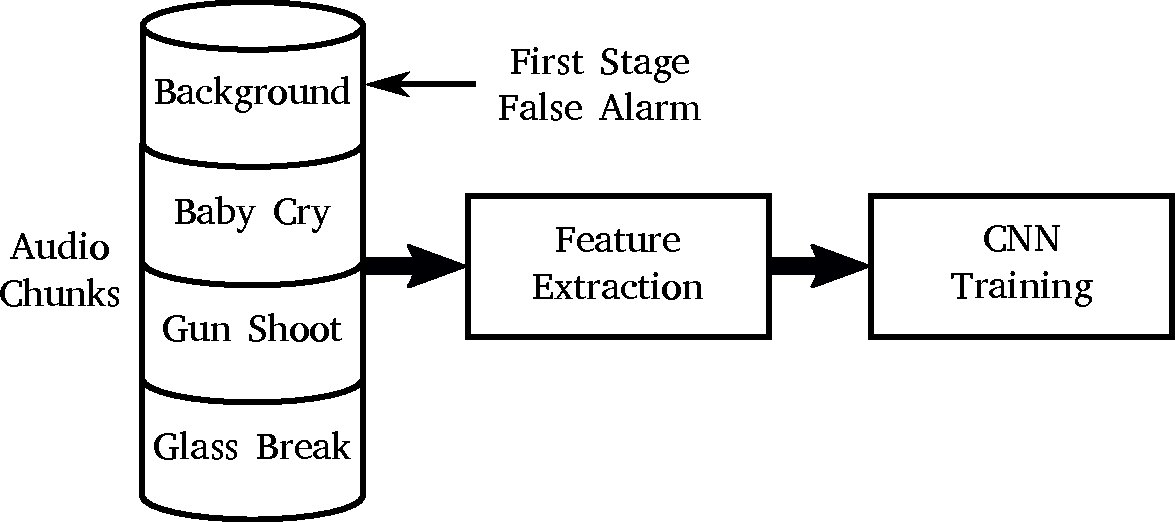
\includegraphics[width=\columnwidth]{Images/training_second_stage.pdf}
	\caption{Training procedure of the CNN-based event detector.}
	\label{fig:CNN-train}
\end{figure}


\subsubsection{Post Processig }
%per ogni seq analizzo tutti gli eventi. Scarto quelli classificati con bck . Prendo il primo evento classificato come non bck perche lo scopo è beccare l onseth
For each audio sequence, we performed the chunk-based CNN classification on the contiguous blocks of frames detected by the MLP event detection stage. Between the frame chunks classified as event by the CNN, %those with the highest network output (which correspond to the probability to belog to the event class) 
the first frame of the contiguous block resulting to have the highest network output average (which correspond to the probability to belog to the event class) was indicated as event onset instant.

\section{Experimental Set-Up}
\label{sec:experiment}
According to the DCASE 2017 guidelines, the performance of the proposed algorithm has been assessed firstly by using the development dataset for training and validation of the system. Then, a blind test on the provided evaluation dataset was performed with the model which achieved the highest performance and submitted to the organizers of the challenge. The performance metric of the DCASE 2017 challenge is the event-based error rate calculated using onset-only condition with a collar of 500 ms. Additionally, event-based F-score with a 500 ms onset-only collar was calculated. Detailed information on metrics calculation is available in \cite{Mesaros2016_MDPI}. The algorithm has been implemented in the Python language using Keras\footnote{https://keras.io/} and Theano \cite{Theano2016short} as deep learning libraries. All the experiments were performed on a computer equipped with a 6-core Intel i7, 32\,GB of RAM and a Nvidia Titan X graphic card.

\subsection{First Event Detection Stage}
%random search per la ricerca di parametri di layout della rete NN: validation split del dcase 
%Per goni rete è stata effettuata un gridsearch sui parametri di post processing per l ottimizzazione del ER
%E' stata selezionata la rete che ha ottenuto l' ER più basso
%La rete selezionata è stata trainata nuovamente con aggiungendo al trainset delle sequenze  contenente gunshot per bilanciare i secondi di materiale degli eventi
The performance of the first event detection stage has been assessed by exploring the networks topology with a random search strategy \cite{bergstra2012random}.
\begin{table}[t]
  \caption{Hyper-parameters optimized in the random-search phase for the onset detection stage, and their range.}\label{tbl:hyper-params-mlp}
  \centering
  \footnotesize
  \begin{tabular} {|c | c | c|}
    \hline
    Parameter & Range & Distribution\\  
    \hline
    \hline                                     
    MLP layers Nr.  & [2 - 7]& uniform \\
    \hline                                     
    MLP layers dim. & [20 - 4048]& log-unifom \\
    \hline                                     
    MLP Context & [3 - 7] & uniform\\
    \hline
    Activation & [tanh - relu] & uniform\\
    \hline
    Dropout & [Yes-No] & uniform\\
    \hline
  \end{tabular}
\end{table}
%%
%
\begin{table}[t]
  \caption{Post processing parameters optimized in grid search phase, and their ranges.}
  \label{tbl:post-proc-params-mlp}
  \centering
  \footnotesize
  \begin{tabular} {|l | c | c |}
    \hline
    Parameter     & Range  & Step\\  
    \hline
    \hline                                     
    Threshold $\theta$ & [0-0.7] & 0.01\\
    \hline                                     
    Window length $M$ & [10-90] & 10 \\
    \hline
    Median filter window $k$ & [9-13] & 2\\
    \hline                                       
  \end{tabular}
\end{table}

% \begin{table}[t]
%   \caption{Hyper-parameters optimized in the random-search phase, and their range.}\label{tbl:hyper-params}
%   \centering
%   \footnotesize
%   \begin{tabular} {|c | c | c|| c | c | c|}
%     \hline
%     Parameter     & Range & Distribution &Parameter & Range & Distribution\\  
%     \hline\hline
%     Cnn layer Nr.   & [1-3]& uniform & Batch size & [10\%-25\%] & log-uniform\\
%     \hline
%     Kernel shape  & [3x3-8x8]& uniform & Max pool shape & [1x1-5x5] & uniform \\
%     \hline                  
%     Kernel Nr.    & [4-64]& log-uniform & Max Pool & All-Only end& uniform \\
%     \hline                                     
%     MLP layers Nr.  & [1-3]& uniform & Dropout & [Yes-No] & uniform\\% dense-layer da uno a tre perchè quello interno ci sta sempre + da 0 a 2 di quelli messi dopo 
%     \hline
%     MLP layers dim. & [128-4096]& log-unifom & Drop rate  & [0.5-0.6] & normal\\
%     \hline
%     Stride & [1x1-3x3]& uniform & Learning rate & [$10^{-4}$-$10^{-2}$]  & log-unifom\\
%     \hline
%   \end{tabular}
% \end{table}

Table \ref{tbl:hyper-params-mlp} shows the parameters explored in the random search, as well as the prior distribution and ranges. 
%%
The number of explored parameters sets depends on the wideness of the search space. In this work, we explored 200 sets of layout parameters for the MLP event detection. The neural networks were trained for 300 epochs on the categorical cross entropy loss function with the Adadelta gradient descent algorithm. The optimizer parameters were set as follows: learning rate $lr=1.0$, $\rho=0.95$, $\epsilon=10^{-6}$.
A successive grid search was performed for each network configuration evaluated in the random seach, in order to find the post-processing parameters that yielded the minimum error rate. Investigated parameters in the grid search were: exponential window length $w$, median filter kernel $k$ and threshold $\theta$. The respective ranges are reported in Table \ref{tbl:post-proc-params-mlp}. The model with resulting minimum error rate was composed as follows: the input layer accepted 120 values for each frame index, corresponding to a context size $C=3$, the hidden layers were two dense layers respectively of size $[631,419]$, to whom the $ReLU$ activation function is applied and finally the output layer is made of two neurons with the softmax function.

Because of the fast decay of the ``gun shot'' sound, we noticed that there was a small amount of audio frames containing this event with respect to the other sound event classes. For this reason we trained the MLP-based event detector obtained from the random seach with an extended dataset, including 500 newly generated mixtures containing the ``gun shot'' sound event.
At the end of the validation stage of the system the neural network was trained including all the mixtures in the development dataset included in the DCASE 2017 challenge package and the aforementioned 500 newly generated containing the ``gun shot'' sound event for a total of 3487 audio sequences. Figure \ref{fig:MLP-train} shows the flow chart of the complete procedure for the MLP-based event detection stage configuration.

\begin{figure}[t]
	\centering
	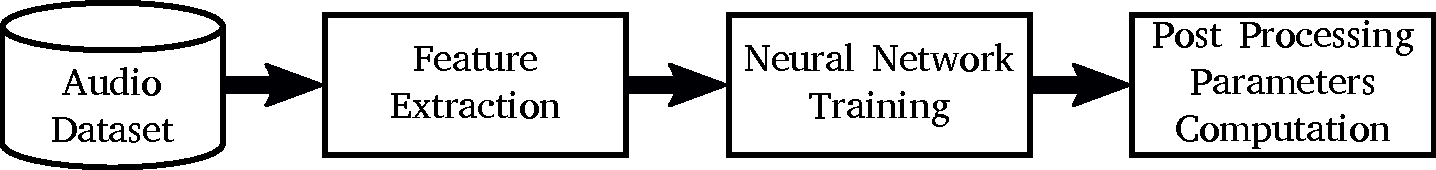
\includegraphics[width=\columnwidth]{Images/training_first_stage.pdf}
	\caption{Set-up procedure of the MLP-based event detection stage.}
	\label{fig:MLP-train}
\end{figure}

\subsection{Multiscaled Refinement Decision Stage}

%Per trainare la cnn abbiamo data in ingresso alla prima rete delle sequenze audio di solo bck. Gli eventi selezionati da questa rete rappresentano il materiale di training
%della classe bck per la cnn. Per le altre classi di eventi abbbiamo preso le porzioni di soli eventi mixed to bck relativi alle mixture fornite dal dcase e gli isolated events.
%
%Abbiamo generato una stratified validation split del dataset appena descritto. 
%Abbiamo effetuato una valutazione della cnn subase evento con la fmeasure.
%Finally, sul validati

To design the best CNN model for our purposes, we generated a shuffle stratified validation split from the dataset composed as described in \ref{ssec:CNN}. We left out the 10\% of the samples as validation set for the CNN model and we selected the layout parameters of the neural network based on the F-measure score obtained on this data sub-set. The best performing model was composed as follows: three convolutional kernel layers respectively with $[16, 8, 8]$ filters each of these of size equal to $3\times3$. Each convolutional layer was followed by a max pooling layer with kernels of size $2\times2$. A dense layer composed of 64 neurons with $tanh$ activation function is applyed before the network output layer. The model was trained for 40 epochs on the categorical cross entropy loss function with the Adadelta gradient descent algorithm with $lr=1.0$, $\rho=0.95$, $\epsilon=10^{-6}$ as for the MLPs.


\subsection{Evaluation Phase}
%Descrizione con img della fase di valutazione
%Scelta th 0.20 invece c he 0.25: per favorile meno deletion a discapito delle insertion. La cnn pensa a eliminare le insertion classificandole come bck
Once the best performing models were found, during the validation stage we performed a fine tuning of the post processing parameters of the MLP-based event detection in order to assess the performance of the whole system. In fact, the hierarchical architecture of the algorithm permits to set a lower threshold in the first decision stage in order to reduce the deletions to the detriment of some insertions. They are removed by the successive decision stage making use of the multi-scale processing acted by the CNN. 
%\textcolor{red}{A complete overview of the parameters of the best performing system are reported in Table YY}. 
It is necessary to notice that in this challenge task the event target class (not its presence or absence) was a prior knowledge, thus in evaluation phase the illustrated procedure is applicable independently to different sequences each potentially containing the respective target event. The final score is then computed overall.
%\textcolor{red}{In table YY are reported the parameters used in each of the four submission that we performed}. 

\section{Results}
\label{sec:results}
\subsection{Results on Development dataset}
The error rate based on the event detection of the first stage on the development dataset is equal to 0.23 and its respective F-measure is 88.0\%. 
After the CNN-based refinement stage, the final overall error rate and F-measure are respectively equal to 0.18 and 90.9\%. 
The post processing parameters used to select the MLP network with the lower ER and the value used in the final evaluation phase are the following:
$\theta=0.20$, $M=70$, $k=11$. 

% \begin{table}[t]
%  \caption{Final Scores. ER stays for only-onset error rate}
%  \label{tbl:finalScore}
%  \centering
%  \footnotesize
%  \begin{tabular} {| c | c | c | c | c |}
%    \hline
%    \multicolumn{2}{c|}{Proposed Method}}& \multicolumn{2}{c|}{Baseline}\\
%    \hline  
%                & ER    &  F-score  & ER    &  F-score  \\  
%    \hline                                     
%    Baby cry    & 0.22  & 89.0 \%      & 0.67  & 72.0 \%\\
%    \hline                                     
%    Glass break & 0.14  & 92.8 \%        & 0.22  & 88.5 \%\\
%    \hline
%    Gun shot    & 0.18  & 91.0 \%        & 0.69  & 57.4 \%\\
%    \hline
%    \textbf{Average} & \textbf{0.18} & \textbf{90.91 \%}& \textbf{0.53} & \textbf{72.7\%}\\
%    \hline                                    
%  \end{tabular}
%\end{table}

 \begin{table}[t] 
 	\caption{Final Scores on Development dataset with $\theta=0.20$, $w=70$, $k=11$.  ER stays for only-onset error rate.}\label{tbl:finalScore} 
 	\centering 
 	\footnotesize 
 	\begin{tabular} {| c | c | c | c | c |} 
 		\hline 
 		& \multicolumn{2}{c|}{Proposed Method}&\multicolumn{2}{c|}{Baseline}\\ 
 		\hline   
 		& ER    &  F-score  & ER    &  F-score  \\   
 		\hline                                      
 		Baby cry    & 0.22  & 89.0 \%      & 0.67  & 72.0 \%\\ 
 		\hline                                      
 		Glass break & 0.14  & 92.8 \%        & 0.22  & 88.5 \%\\ 
 		\hline 
 		Gun shot    & 0.18  & 91.0 \%        & 0.69  & 57.4 \%\\ 
 		\hline 
 		\textbf{Avarage} & \textbf{0.18} & \textbf{90.91 \%}& \textbf{0.53} & \textbf{72.7\%}\\ 
 		\hline 
 		
 	\end{tabular} 
 	
 \end{table} 


With respect to the DCASE 2017 baseline system the improvement in terms of error rate reduction is equal to 0.35. In Table \ref{tbl:finalScore} are reported the scores for the two stages of the proposed system and the baseline.

\subsection{Results on Evaluation dataset}
The parameters used for the different submitted systems for the task 2 of DCASE 2017 challenge are reported in table \ref{tbl:submitted-params}.

\begin{table}[t]
	\caption{Post processing parameters for submitted systems. Only the threshold is varied, $M = 70$ and $k=11$.}
	\label{tbl:submitted-params}
	\centering
	\footnotesize
	\begin{tabular} {| c | c |}
		\hline
		Parameter     & Submission label\\  
		\hline
		\hline                                     
		$\theta=0.18$ & Vesperini\_UNIVPM\_task2\_1 \\
		\hline                                     
		$\theta=0.198$ & Vesperini\_UNIVPM\_task2\_2 \\
		\hline
		$\theta=0.20$ & Vesperini\_UNIVPM\_task2\_3 \\
		\hline   
		$\theta=0.22$ & Vesperini\_UNIVPM\_task2\_4 \\
		\hline                                       
	\end{tabular}
\end{table}


\subsection{Real Scenario application}
%Descrizione scenario reale: trainig cnn su 4 classi
%risultato finale 0.23
%non metterei in tabella perchè farebbe confusione,  magari in un extended paper lo faremo
In our investigation we evaluated also a system applicable in a real word scenario, where the event target class is not knowable in advance. In this case the role of the CNN-based stage other than refine the MLP-based event detection is also to classify the event class. For this setup we achieved an overall error rate equal to 0.23 and a respective F-measure of 90\%.

\section{Conclusion and Outlook}
\label{sec:conclusion}
 In this paper, a hierarchic multi-scaled neural network based approach for rare sound event detection is presented.  We extracted acoustic features from the audio signals, then the event detection is performed by an MLP-based stage and refined by a CNN-based decision stage, each with dedicated post processing procedures. To assess the performance of the algorithm we conducted experiments on the development dataset from the DCASE 2017 setup. According to the challenge specifications, the performance of the system are evaluated in terms of event-based error rate calculated using onset-only condition with a collar of 500 ms on the validation subset, achieving an error rate on the Development dataset equal to 0.23 with respect to an error rate equal to 0.53 of the baseline system. On the blind evaluation dataset, the best setup between 4 different threshold values achieves an error rate equal to 0.33 and an F-measure equal to 83.9\%.
 
Future work will comprise the exploitation of event dedicated acoustic features, to better focus on the distinctive tracts given by the heterogeneous nature of the events. A deeper focus will be given also to the temporal evolution of the signal by means of recurrent structure, such as Long Short Term Memory (LSTM) Neural Networks \cite{hochreiter1997long}.
%

% -------------------------------------------------------------------------
% Either list references using the bibliography style file IEEEtran.bst
\bibliographystyle{IEEEtran}
\bibliography{refs}
%


\end{sloppy}
\end{document}
\grid
